\documentclass[12pt]{article}
\usepackage[margin=1in]{geometry}
\usepackage{amssymb}
\usepackage{graphicx}
\setlength{\parindent}{0pt}

\title{Flow Models - Notes}
\author{Devesh Nath}
\date{\today}
\begin{document}

\maketitle

\section{Learning Robotic Manipulation Policies from Point Clouds with Conditional Flow Matching}
\begin{figure}[h!]
    \centering
    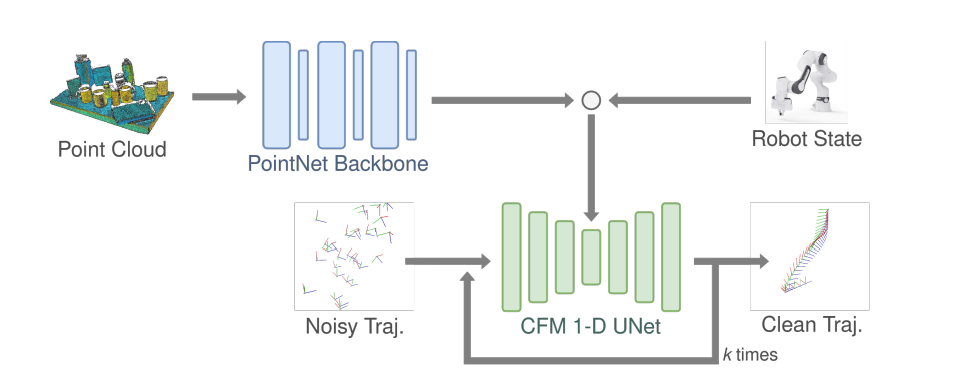
\includegraphics[width=0.7\textwidth]{1.png}
    \label{fig:example_image}
\end{figure}
Expert demonstrations encode the goal state. From random starting states, actions re collected.
The policy learns to "flow" a noisy trajectory to the clean trajectory.
The pointcloud information is encoded using PointNet and the robot state is also provided to the CFM policy. 
They try SO(3) and Euclidean R(6) formulation. The euclidean worked better, may be due to disconitnuities in SO(3). 
They use 2 Real-Sense cameras in real life, merge pointclouds and run the policy. Achieved a success rate of 72\% for open box and 48\% for sponge on plate. Failure mode was basicall robot missing by a fmall margin. 
\begin{figure}[h!]
    \centering
    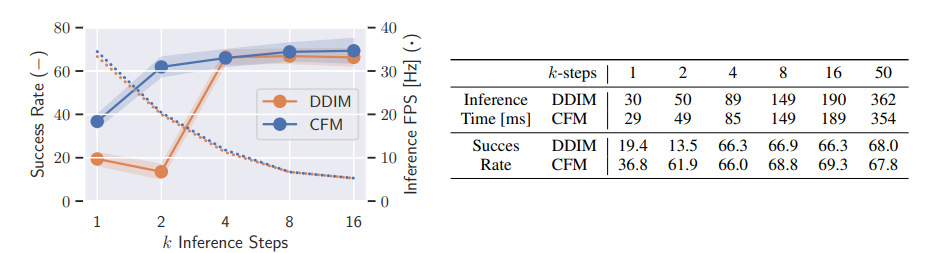
\includegraphics[width=0.7\textwidth]{2.png}
    \label{fig:second_image}
\end{figure}

\newpage
\section{Questions/Ideas/Notes}
\begin{itemize}
    \item AdaFlow has a variance estimation network to predict the variance of the current state and adjusts the number of integration steps dynamically to reduce inference time. 
    \item What is differentiable sim? Can it be used directly to train flow models (that output gradients)?
    \item Neural ODES and conditional flow models predict $\frac{dx}{dt} = f_{\theta}(x, t)$. Is there a way to integrate control such that $\frac{dx}{dt} = f_{\theta}(x, u, t)$.
    \item ControlSynth Neural ODEs. 
    \item Latent flow models? If we have a VAE bottlenecking the flow model, we can get mean and std deviation of the latent state. Probabilisttic bounds on the output trajectory using this? Better generalization?
    \item Just in time computation with CFM or Diffusion?
\end{itemize}

\end{document}